% !TeX root = ../XMU.tex
\chapter{实证分析}{Analysis of Model Empirical Results}

%加上一个Z就不显著,说明Z可能与X强相关

% 通过对上市公司不同板块的分类,我们可以得到如\cref{board_fraud}所示
% \begin{figure}[!ht]
%     \centering
%     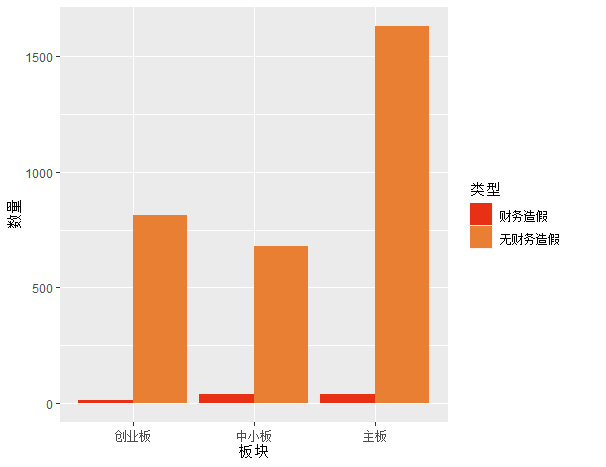
\includegraphics[scale=1]{Board_fraud}
%     \caption{不同板块的财务造假统计} \label{board_fraud}
%     \end{figure}
% 可以看到在不同的板块,财务造假的公司分类的还是比较均匀的,没有在某个板块财务造假的现象极为突出的情况存在

\section{数据平衡与样本重建}{Data Balance and Sample Reconstruction}
初步我们得到有极强的造假嫌疑的样本共120个,无造假嫌疑的样本有3088个,二者比例为1:25左右,存在较为严重的样本不平衡问题。对于这个问题的解决主要通过欠采样和过采样的方法,考虑到欠采样将导致样本的数据急剧下降,因此本文采用的过采样的方法进行解决。

本文采用SMOTE方法\cite{Chawla2011SMOTE}进行数据过采样,最终得到造假样本440条,非造假样本528条,二者比例接近1:1。

\section{Logistic模型实证分析}{Logistic Model Empirical Analysis}
\subsection{Logistic模型}{Logistic Model}
Logistic 回归模型是传统经典的分类方法,在因变量取值为二分类时进行回归分析,基本思路是通过 Logistic 非线性变换,利用极大似然估计的方法,通过Newton-Raphson方法进行迭代求解,求出系数的估计值,建立一个概率拟合函数。它是一个参数线性的判别类,用于解释一个二元变量与一个或多个度量自变量之间的关系 
\cite{agresti_introduction_2007}。


本文通过 Logistic 回归模型将自变量的取值代入到概率拟合函数,在二元值中通过预测因变量的概率取值,假设预测概率大于 0.5,则财务舞弊预测发生,预测概率小于 0.5,则财务造假预测不发生。概率取值为度量尺度,从而判断样本的所属类别进行二分类。

\subsection{Logistic模型的构建与实证分析}{Logistic Model Construction and Empirical Analysis}

%作这些回归的目的,探究中国上市公司的主要造假手段,以及在财务类高管领取与不领取报酬的公司,相同的造假手段是否存在异质性
%之前会报错的原因是下划线忘记用斜杠转义了

首先本文先对前文提到的变量共17个\footnote{排除了两个共线性变量liquidity\_ratio与capital\_preservation。},
进行建模得到一个完整的全模型,而后,根据AIC原则,采用向前和向后两种变量选择方法得到了相同的结果,再删除掉不显著的无关变量,最终得到了如表\ref{logistic_regression}中的方程(1),该方程的变量选择涉及到了我们所构建指标的各个方面,其中财务表现,发展能力,治理结构,动力指标,偿债能力这几个方面都有变量入选。

表\ref{logistic_regression}汇报了基于先前初步选择变量的结果。从方程(1)可以看出,在财务造假的表现方面,operationg\_cost显著为负的,即营业总成本增长,对于财务造假的预测具有明显的负效应。换句话说,中国的上市公司在财务造假的过程中,往往会选择通过即营业总成本减少以达到虚增利润的效果,而较少会通过计提坏账准备,减少销售费用和减少管理费用的方式;在发展能力方面sustain\_grow\_rate是显著为负的,而且其对最终财务造假的预测影响较大,说明一个发展前景较好的公司具有较低的财务造假的可能,这与之前的理论分析相契合;

% 在公司的治理结构方面,TopTenHolderRate的系数是显著为负的,说明从整个市场的来看,前十大股东的持股比例越高,其财务造假的风险反而越低,这与我们先前的理论似乎相违背,但是该指标的系数大小仅为

在方程(1)中财务类高管是否领取薪酬对于财务造假的预测是没有显著影响的,然而作为动力指标,不领取薪酬可能会导致更强的财务嫌疑,因为其报酬极有可能与公司的财务表现相挂钩,其主观动力会更强。

为探究在不同的财务指标下,财务类高管领取与不领取薪酬对财务造假是否存在不同影响,得到了回归方程(2)加入了get\_paid与quick\_ratio的交叉项,可以知道,财务类高管领取薪酬确实对财务造假预测有一定的影响,且其参数显著为负,表明财务类高管没有在上市公司领取薪酬,将会使降低财务报表造假预测的概率,即认为财务类高管没有领取薪酬的上市公司财务造假的可能会小于那些财务类高管领取薪酬的上市公司,并且该影响将会随着quick\_ratio的上升而弱化,当$quick\_ratio>1.318$,该影响将会由负转正。
% 对比方程(2)与方程(3)可以发现财务类高管领取薪酬对是否财务造假存在simpson悖论,即从整个中国上市公司整体环境来看,财务类高管领取薪酬对财务造假影响不显著,但是在不同的速动比率的公司,财务类高管是否领取薪酬对上市公司是否财务造假具有显著的影响,甚至随着速动比率的不断上升,其影响会由负转正。
速动比率衡量的是短期偿债能力,从衡量长期偿债能力的assets\_liabilities即资产负债率来看,结论也是类似的。速动比率是一个正向指标\footnote{正向指标指认为指标值越大,偿债能力越强,负向指标与之相反},资产负债率是一个负向指标。因此,同样对比方程(1)与方程(3)可以发现在不同资产负债率的公司,财务类高管是否领取薪酬对上市公司是否财务造假具有显著的影响,甚至随着资产负债率的不断上升,其影响会由正转负。因此这就说明了观点:在不同偿债能力的公司,财务类高管是否领取薪酬对上市公司是否财务造假具有显著的影响是不同的,偿债能力越强的公司,其财务类高管领取薪酬对财务造假的预测具有更强的负向影响,即认为财务类高管领取薪酬会减少财务造假的可能,而且这种影响在偿债能力强的公司将会更加显著。








%这个公式mathtype那边剪切格式要改一下,太长了


%R语言实证结果,需要将tabular改为longtable,并把前面的一些table内容删掉,并且要注意,tabular的东西只能放在一个页面当中
% 然后标题和label要用\caption{\label{tab:test}我的跨页表格}的格式写
% 通过\renewcommand\arraystretch{0.5}来调整行距,0.5就挺好的

\renewcommand\arraystretch{0.5}
  \begin{longtable}{@{\extracolsep{5pt}}lD{.}{.}{-3} D{.}{.}{-3} D{.}{.}{-3} } 
    \caption{\label{logistic_regression}回归结果}
    \\[-1.8ex]\hline 
    \hline \\[-1.8ex] 
     & \multicolumn{3}{c}{\textit{Dependent variable:}} \\ 
    \cline{2-4} 
    \\[-1.8ex] & \multicolumn{3}{c}{ViolationTypeID} \\ 
    \\[-1.8ex] & \multicolumn{1}{c}{(1)} & \multicolumn{1}{c}{(2)} & \multicolumn{1}{c}{(3)}\\ 
    \hline \\[-1.8ex] 
     get\_paid2 & 0.484 & -1.566^{**} & 2.863^{**} \\ 
      & (0.407) & (0.774) & (1.250) \\ 
      & & & \\ 
     quick\_ratio & 0.177^{***} & 0.160^{***} & 0.176^{***} \\ 
      & (0.061) & (0.059) & (0.060) \\ 
      & & & \\ 
     assets\_liabilities & 1.421^{**} & 1.525^{**} & 1.571^{**} \\ 
      & (0.632) & (0.630) & (0.637) \\ 
      & & & \\ 
     cash\_liabilities & -2.343^{***} & -2.371^{***} & -2.400^{***} \\ 
      & (0.475) & (0.480) & (0.479) \\ 
      & & & \\ 
     sustain\_grow\_rate & -7.302^{***} & -7.329^{***} & -7.321^{***} \\ 
      & (0.709) & (0.712) & (0.711) \\ 
      & & & \\ 
     TopTenHoldersRate & -0.012^{**} & -0.011^{*} & -0.011^{*} \\ 
      & (0.006) & (0.006) & (0.006) \\ 
      & & & \\ 
     operating\_cost & -0.361^{*} & -0.333^{*} & -0.319^{*} \\ 
      & (0.208) & (0.188) & (0.187) \\ 
      & & & \\ 
     get\_paid2:quick\_ratio &  & 1.188^{***} &  \\ 
      &  & (0.438) &  \\ 
      & & & \\ 
     get\_paid2:assets\_liabilities &  &  & -5.151^{**} \\ 
      &  &  & (2.517) \\ 
      & & & \\ 
     Constant & -0.249 & -0.309 & -0.353 \\ 
      & (0.512) & (0.510) & (0.514) \\ 
      & & & \\ 
    \hline \\[-1.8ex] 
    Observations & \multicolumn{1}{c}{968} & \multicolumn{1}{c}{968} & \multicolumn{1}{c}{968} \\ 
    Hosmer-Lemeshow X2 & \multicolumn{1}{c}{$47.229^{***}$} & \multicolumn{1}{c}{$48.862^{***}$} & \multicolumn{1}{c}{$47.947^{***}$} \\ 
    \hline 
    \hline \\[-1.8ex] 
    \textit{Note:}  & \multicolumn{3}{r}{$^{*}$p$<$0.1; $^{**}$p$<$0.05; $^{***}$p$<$0.01} \\  
  \end{longtable} 




\subsection{Logistic模型评价}{Logistic Model Evaluation}
本文通过变量选择得到了模型\cref{eq:last}其方程为:
  
% \[\begin{array}{ccccc}
%     \log it(\hat \pi ) =&- 0.0651 + 0.1544quick\_ratio + 1.2126assets\_liabilities\\
%     &  - 2.0919cash\_liabilities - 0.2404asset\_turnover\\
%      &  - 6.2771sustain\_grow\_rate - 0.00136TopTenHoldersRate\\
%      &+1.3843get\_paid + 0.2187management\_rate
%     \end{array}\]

\begin{equation}
    \begin{aligned}
        \log it(\hat \pi ) =&- 0.309 + 1.566get\_paid+0.160quick\_ratio + 1.525assets\_liabilities\\
    &- 2.371cash\_liabilities- 7.329sustain\_grow\_rate - 0.011TopTenHoldersRate\\
        &-0.333operating\_cost+1.188get\_paid2\times quick\_ratio
    \end{aligned} 
    \label{eq:last}   
\end{equation}

其中:$\log it(\hat \pi ) = ln(\frac{{\hat \pi }}{{1 - \hat \pi }})$

对上述模型,本文选择了常用的auc指标与混淆矩阵\footnote{其中$\pi_{0}$为样本比例0.545}对其预测能力进行评判。根据模型可得到如\cref{ROC}所示的ROC曲线图,其AUC值达到了0.8834,具有较好的识别财务造假的能力。为使得到的结果更加具有稳健性,本文接着采用了十折交叉检验\footnote{即将所有的数据随机切割成十份,依次选择其中九份作为训练集,剩下一份样本为测试集}的方式对样本进行切割为训练集和测试集,用训练集拟合模型参数,并用训练集进行检验预测能力,并将得到的混淆矩阵十次的结果取平均,得到如\cref{Confusion matrix}所示,其specificity的均值为0.911,sensitivity的均值为0.702,十次得到的auc取均值为0.886。综上,是可以认为我们建立得到的模型是具有较强的预测能力的。

\begin{figure}[!ht]
    \centering
    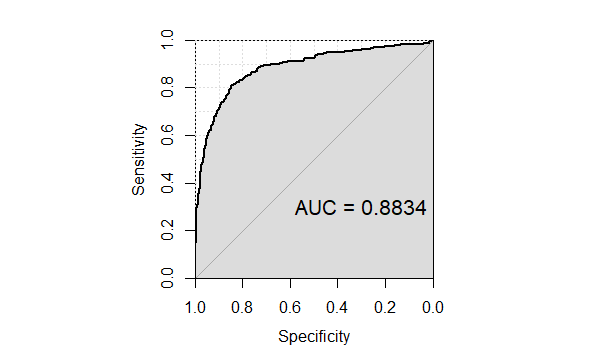
\includegraphics[scale=1]{ROC}
    \caption{logistic ROC} \label{ROC}
    \end{figure}

    % Please add the following required packages to your document preamble:
% \usepackage{multirow}
\begin{table}[!ht]
    \centering
    \caption{Confusion matrix}
    \label{Confusion matrix}
    \begin{tabular}{ccc}
        \toprule
    \multirow{2}{*}{Fraud In Reality} & \multicolumn{2}{c}{Fraud In Prediction} \\ \cline{2-3} 
                                      & T                  & F                  \\ \toprule
    T                                 & 40.0               & 3.9                \\
    F                                 & 15.5               & 36.6               \\ \bottomrule
    \end{tabular}
    \end{table}


\section{随机森林模型分析}{Random Forest Model Analysis}

为探究本文选择的变量在使用其他预测模型时仍然有较好的效果,本文选择了树模型对本文选择的变量进行预测,%下面这句是抄的
树模型包括决策树,随机森林,提升树等,其中随机森林(Randomforest),提升树作为一种组合分类器算法,在大样本、高维度特征和异常值数据上仍然能够保持较好的预测准确率,最终通过准确率的比较,本文选择了随机森林模型作为最终模型,在这项预测中,随机森林模型在多种树模型中具有明显的优点。

\subsection{随机森林模型}{Random Forest Model}
随机森林模型通过对树作相关处理,实现对袋装法树的改进。在随机森林中需对自助抽样训练集建立一系列决策树,但是在建立决策树时,每考虑树上的一个分裂点,都要从全部的p个预测变量中选出一个包含m个预测变量的随机样本作为候选变量。随机森林算法可以用于连续变量的预测,也可以用于分类型变量的预测,对于本文的二值变量的预测同样具有较好的效果\cite{james_introduction_2013}。
随机森林模型的决策树分类器的构建过程如下:
%抄的

(1)对原始数据集有放回的随机抽样,引导生成与原始实例集相同数量的样本,组成一定规模的随机子集,随机子集的规模对应随机森林的规模;

(2)在每个随机子集的生成过程中,可以证明,约有37\%的样本不会被采用,称为OOB(out of bagging)。并且,利用OOB进评估模型的训练损失,是一种无偏估计\cite{Breiman2001Random}。


(3)随机子集对应决策数根节点。在每个节点随机抽样样本特征,最后到达限制层数或者当每个叶节点是纯数据的时候,停止分裂。

\subsection{随机森林模型的选择与构建}{Selection and Construction of Random Forest Model}
本文采用前文提到的十折交叉验证来对进行模型的选择,通过对树的棵树进行调参,并采用十折交叉验证来计算其平均的准确度,最终得到三种模型的准确率的对比如图\ref{three_model}。从图中可以到随机森林算法的误差率是显著小于Bagging和Adaboost的,故最终选择了随机森林算法,找到其中使误差最小的树的棵数为505。
\begin{figure}[!ht]
    \centering
    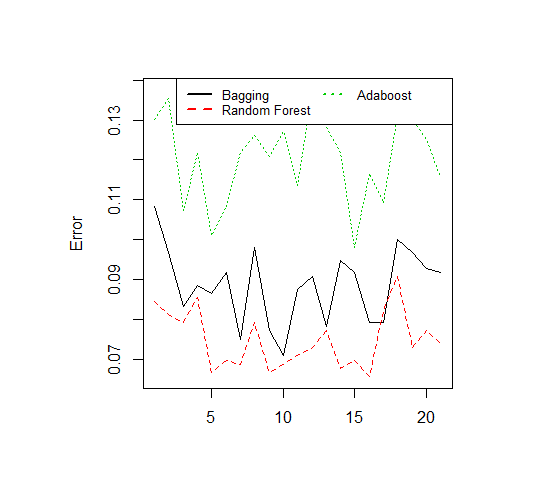
\includegraphics[scale=1]{three_model}
    \caption{模型平均误差图} \label{three_model}
    \end{figure}


\subsection{随机森林模型的评价}{Random Forest Model Evaluation}

使用准确率最高的参数即$ntree = 505$,$mtry = 4$建立随机森林模型可以得到其准确率达93.4\%。

对于上述模型,本文同样选择了常用的auc指标与混淆矩阵对其预测能力进行评判。根据模型可以得到如图\ref{randomforest_ROC}所示的ROC曲线,其AUC值达到了0.976,相对于logistic模型来说是显著的提升。同样使用十折交叉检验的方式对样本进行切割,并得到十次的平均混淆矩阵,得到如表\cref{confusion_}所示,其specificity的均值为0.900,sensitivity的均值为0.914,相对于logistic模型来说,其specificity的值没有明显的下降,但是sensitivity却有明显的提高。


\begin{figure}[!ht]
    \centering
    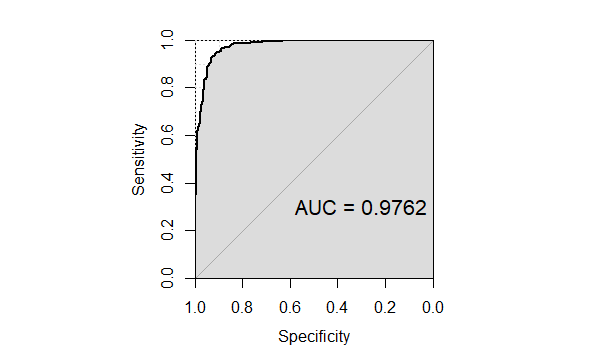
\includegraphics[scale=1]{randomforest_ROC}
    \caption{RandomForest ROC} \label{randomforest_ROC}
    \end{figure}

    % Please add the following required packages to your document preamble:
% \usepackage{multirow}
\begin{table}[!ht]
    \centering
    \caption{Confusion matrix}
    \label{confusion_}
    \begin{tabular}{ccc}
    \hline
    \multirow{2}{*}{Fraud In Reality} & \multicolumn{2}{c}{Fraud In Prediction} \\ \cline{2-3} 
                                      & T                  & F                  \\ \hline
    T                                 & 38.0               & 4.2                \\
    F                                 & 4.6                & 49.2               \\ \hline
    \end{tabular}
    \end{table}


对于随机森林模型为什么可以显著提高sensitivity的原因除了该模型可以解决非线性分类等模型本身的优势之外,其预测变量的选择与logistic模型选择的变量不同也是重要的一方面,如图\ref{importance}所示,可以看到在随机森林模型判别标准中利润总额增长率和可持续增长率是判别模型中最重要的变量,其中利润总额增长率在logistic模型甚至没有出现在最终选择的模型中。


\begin{figure}[!ht]
    \centering
    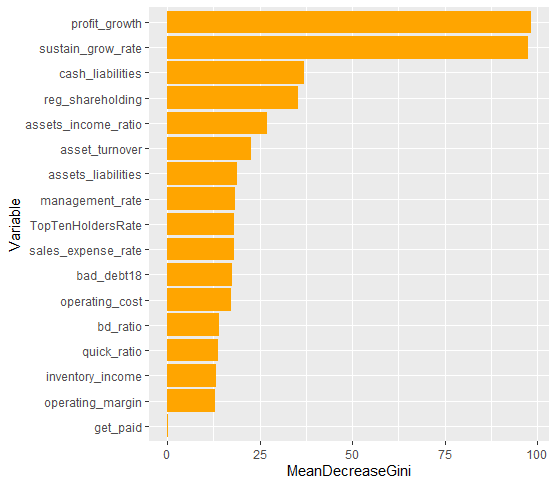
\includegraphics[scale=1]{importance}
    \caption{变量重要性排序} \label{importance}
    \end{figure}